\documentclass{beamer}
\usetheme{Madrid}

%packages
\usepackage{graphicx}
\usepackage{tikz}
\usepackage{subcaption}
\usepackage{amsmath}
\usepackage{amssymb}
\usepackage{bbm}
\usepackage{mathtools}
\usepackage{parskip}
\usepackage{xcolor}
\usepackage[numbers, compress]{natbib}
\bibliographystyle{plainnat}

%graphics
\graphicspath{{./img/}}

%custom commands
\newcommand{\Fcal}{\mathcal{F}}
\newcommand{\Dcal}{\mathcal{D}}
\newcommand{\Gaussian}{\mathcal{N}}
\newcommand{\Lcal}{\mathcal{L}}
\newcommand{\Tcal}{\mathcal{T}}
\newcommand{\one}{\mathbbm{1}}
\DeclareMathOperator*{\argmax}{arg\,max} % Jan Hlavacek
\DeclareMathOperator*{\argmin}{arg\,min} % Jan Hlavacek
\def\imagebox#1#2{\vtop to #1{\null\hbox{#2}\vfill}}

\title{Inferring community characteristics in labelled networks}
\subtitle{IIB Project}
\author{Lawrence Tray}
\institute{Ioannis Kontoyiannis}
\date{\today}

%\AtBeginSection[]{
%	\begin{frame}
%		\vfill
%		\centering
%		\begin{beamercolorbox}[sep=8pt,center,shadow=true,rounded=true]{title}
%			\usebeamerfont{title}\insertsectionhead\par%
%		\end{beamercolorbox}
%		\vfill
%	\end{frame}
%}

\begin{document}
	
	%title
	\begin{frame}
		\titlepage
	\end{frame}

	\begin{frame}{Overview}
		\tableofcontents
	\end{frame}

\section{Introduction}
	
	\begin{frame}{Let's define some terms}
		\begin{block}{Inferring community characteristics in labelled networks}
			\begin{description}
				\item[Network] set of vertices (aka nodes) connected by edges.
				\item[Graph] same as a network.
				\item[Labelled] information about each vertex. We call these {\em features}.
				\item[Community] densely connected subset of nodes.
				\item[Block] same as a community.
			\end{description}
		\end{block}
		\centering
		\vspace{1cm}
		Aim to identify how {\em features} impact graphical structure
	\end{frame}
	
	\begin{frame}{How we got here}
		\begin{itemize}
			\item Started by performing hypothesis tests on features 
		\end{itemize}
		
		\begin{figure}
			\begin{subfigure}{0.4\linewidth}
				\centering
				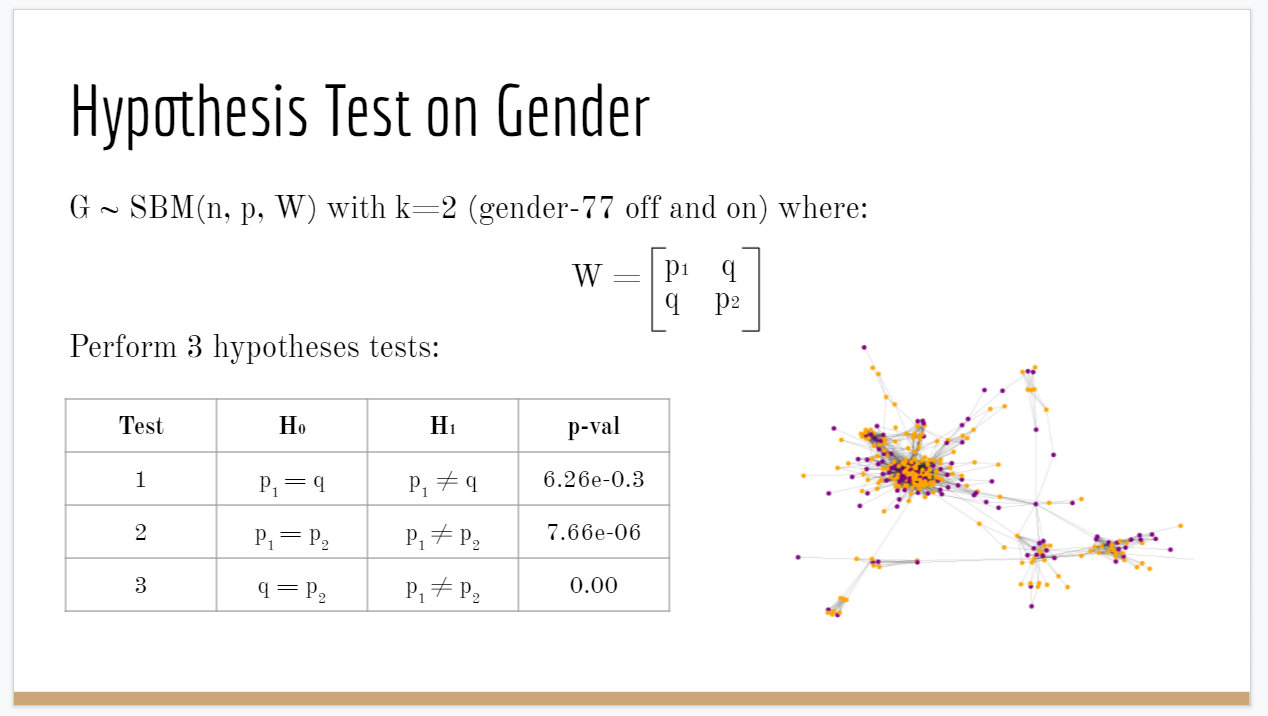
\includegraphics[width=\linewidth]{old-presentation-0}
			\end{subfigure}
			\begin{subfigure}{0.4\linewidth}
				\centering
				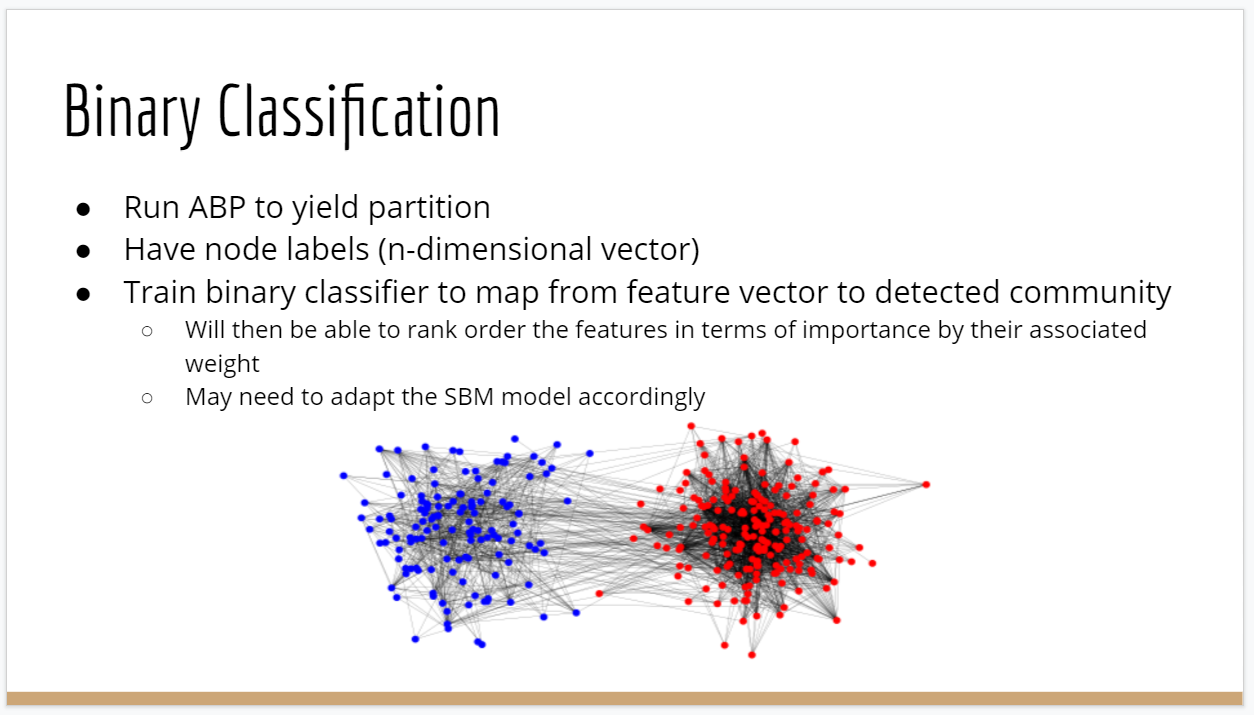
\includegraphics[width=\linewidth]{old-presentation}
			\end{subfigure}
			\caption{Slides from Michaelmas presentation}
		\end{figure}
	
		\begin{itemize}
			\item This proved unhelpful as:
			\begin{itemize}
				\item Almost all features statistically significant
				\item Hard to rank order features against one another
				\item Often poor model fit
			\end{itemize}
		\end{itemize}
	
		\begin{block}{}
			Instead: find most ``natural" partition and see if features can explain
		\end{block}
	\end{frame}

\section{Preliminaries}
	
	\begin{frame}{The stochastic block model (SBM)}
		We adopt the degree-corrected (DC) microcanonical (MC) formulation \cite{Peixoto-Bayesian-Microcanonical}.				
		\begin{columns}
			
			\column{0.5\textwidth}
			
			\begin{itemize}
				\item $N$ -- number of vertices
				\item $B$ -- number of blocks
			\end{itemize}
			\vspace{0.3cm}
			DC-SBM$_{\textrm{MC}}$ parameters:
			\begin{itemize}
				\item $b$ -- block membership vector
				\item $e$ -- block connectivity matrix
				\item $k$ -- degree sequence
			\end{itemize}
			
			$$A \sim \textrm{DC-SBM}_{\textrm{MC}}(b, e, k)$$
			
			\column{0.5\textwidth}
		
			\begin{figure}
				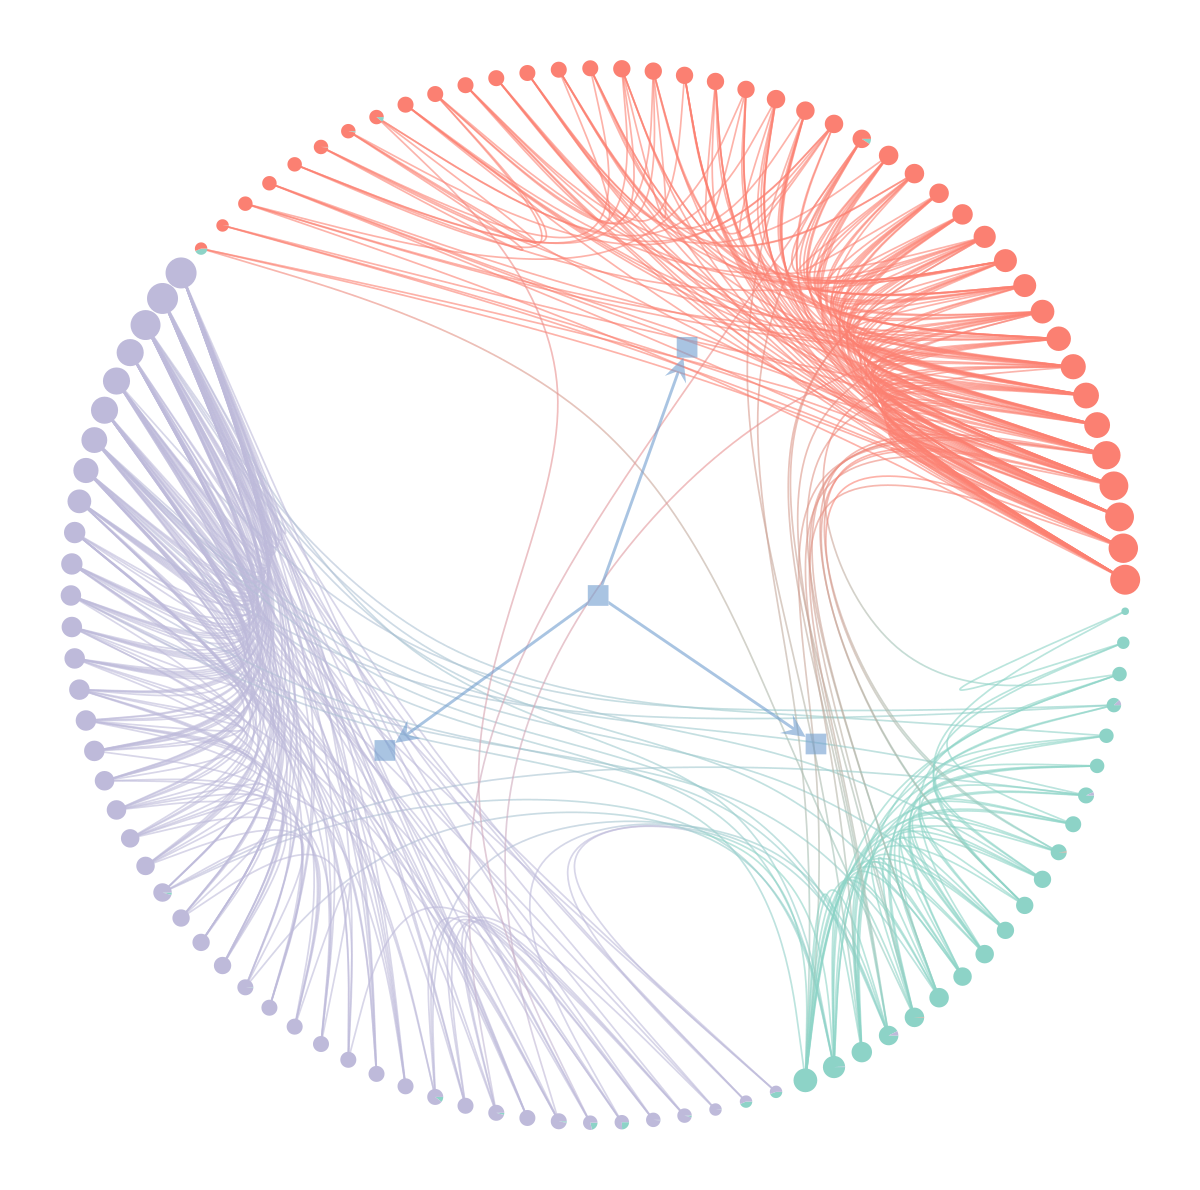
\includegraphics[width=0.6\linewidth]{polbooks-graph}
				\caption{Typical SBM graph}
			\end{figure}
		\end{columns}
		With edges placed uniformly at random but respecting:
		\begin{equation*}
			e_{rs} = \sum_{i, j \in [N]} A_{ij} 
			\one \{b_i = r\} \one \{b_j = s\} 
			\qquad 
			\textrm{and} \qquad
			k_i = \sum_{j \in [N]} A_{ij}.
			\label{eqn:sbm-constraints}
		\end{equation*}
	\end{frame}

\section{The feature-first block model}

	\begin{frame}{The feature-first block model (FFBM)}
		Define feature matrix $X \in \{0, 1\}^{N \times D}$, this gives us that:
		\begin{figure}[!h]
			\centering
			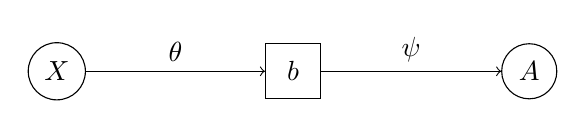
\begin{tikzpicture}[
				roundnode/.style={circle, draw=black, minimum size=7mm},
				squarednode/.style={rectangle, draw=black, minimum size=7mm}
				]
				% nodes
				\node[roundnode] (X) at (0, 0) {$X$};
				\node[squarednode] (b) at (3, 0) {$b$};
				\node[roundnode] (A) at (6, 0) {$A$};
				
				% arrows
				\draw[->] (X.east) -- node[above] {$\theta$} (b.west);
				\draw[->] (b.east) -- node[above] {$\psi$}(A.west);
			\end{tikzpicture}
			\caption{The feature-first block model (FFBM)}
			\label{fig:ffbm}
		\end{figure}
	
		\begin{columns}
			\column{0.55\textwidth}
			\begin{block}{Likelihoods}
				$$p(b|X; \theta) = \prod_{i \in [N]} \phi_{b_i} (x_i; \theta)$$
				$$p(A|b; \psi) \sim \textrm{DC-SBM}_{\textrm{MC}} (b, \psi_e, \psi_k)$$
			\end{block}
		
			\column{0.4\textwidth}
			\begin{block}{Priors}
				$$p(\theta) = \Gaussian(\theta;0, \sigma_\theta^2 I)\vspace{4mm}$$
				$$p(\psi | b) = p(\psi_e | b) p(\psi_k | \psi_e, b)$$
			\end{block}
		\end{columns}
	
		\vspace{5mm}
		$$\phi_{j}(x; \theta) \coloneqq \frac{\exp (w_j^T x_i)}{\sum_{k \in [B]} \exp (w_k^T x_i) }$$
	\end{frame}

	\section{Inference}
	\begin{frame}{Inference procedure}
		We want to draw:
		$$\theta^{(t)} \sim p(\theta| A, X).$$
		But computing $p(A| \theta, X)$ is $O(B^N) \Rightarrow$  split into:
		\begin{align*}
			b^{(t)} &\sim p \Big( b| A, X \Big) \\
			\theta^{(t)} &\sim p \Big( \theta| X, b^{(t)} \Big)
		\end{align*}
		Both steps implemented through Metropolis-Hastings, with:
		$$\pi_z(z) \textrm{ -- target } \qquad q_z(z, z') \textrm{ -- proposal } \qquad \alpha_z(z, z') \textrm{ -- accept prob}$$		
	\end{frame}
	
	\begin{frame}{Sampling sequence}
		\begin{figure}[!h]
			\centering
			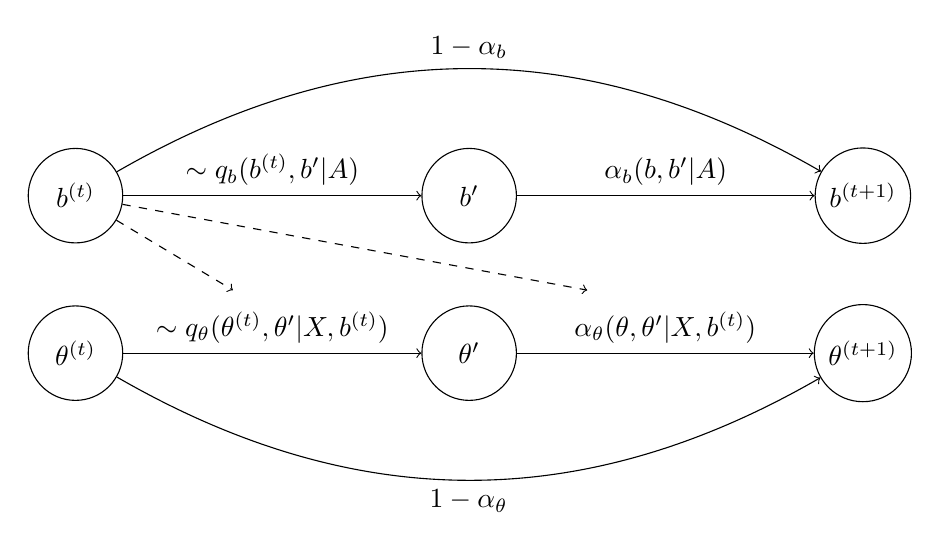
\begin{tikzpicture}[
				scale=1.0, every node/.style={transform shape},
				roundnode/.style={circle, draw=black, minimum size=12mm},
				squarednode/.style={rectangle, draw=black, minimum size=12mm}
				]
				% nodes
				\node[roundnode] (b0) at (0, 2) {$b^{(t)}$};
				\node[roundnode] (b1) at (5, 2) {$b'$};
				\node[roundnode] (b2) at (10, 2) {$b^{(t+1)}$};
				\node[roundnode] (t0) at (0, 0) {$\theta^{(t)}$};
				\node[roundnode] (t1) at (5, 0) {$\theta'$};
				\node[roundnode] (t2) at (10, 0) {$\theta^{(t+1)}$};
				
				% arrows
				\draw[->] (b0) to node[above] {$\sim q_b(b^{(t)}, b' | A)$} (b1);
				\draw[->] (b1) to node[above] {$\alpha_b (b, b' | A)$} (b2);
				\draw[->] (b0) [out=30, in=150] to node[above] {$1-\alpha_b$} (b2);
				
				\draw[->] (t0) to node[above] {$\sim q_\theta(\theta^{(t)}, \theta' | X, b^{(t)})$} (t1);
				\draw[->] (t1) to node[above] {$\alpha_\theta (\theta, \theta' | X, b^{(t)})$} (t2);
				\draw[->] (t0) [out=-30, in=-150] to node[below] {$1-\alpha_\theta$} (t2);
				
				\draw[dashed, ->] (b0) to (2, 0.8);
				\draw[dashed, ->] (b0) to (6.5, 0.8);
				
			\end{tikzpicture}
			\caption{Sampling sequence.}
			\label{fig:samp-sequence}
		\end{figure}
	\end{frame}

\section{Experiments}

	\begin{frame}{The datasets}
		\begin{figure}[!h]
			\centering
			\begin{subfigure}[t]{0.3\linewidth}
				\centering
				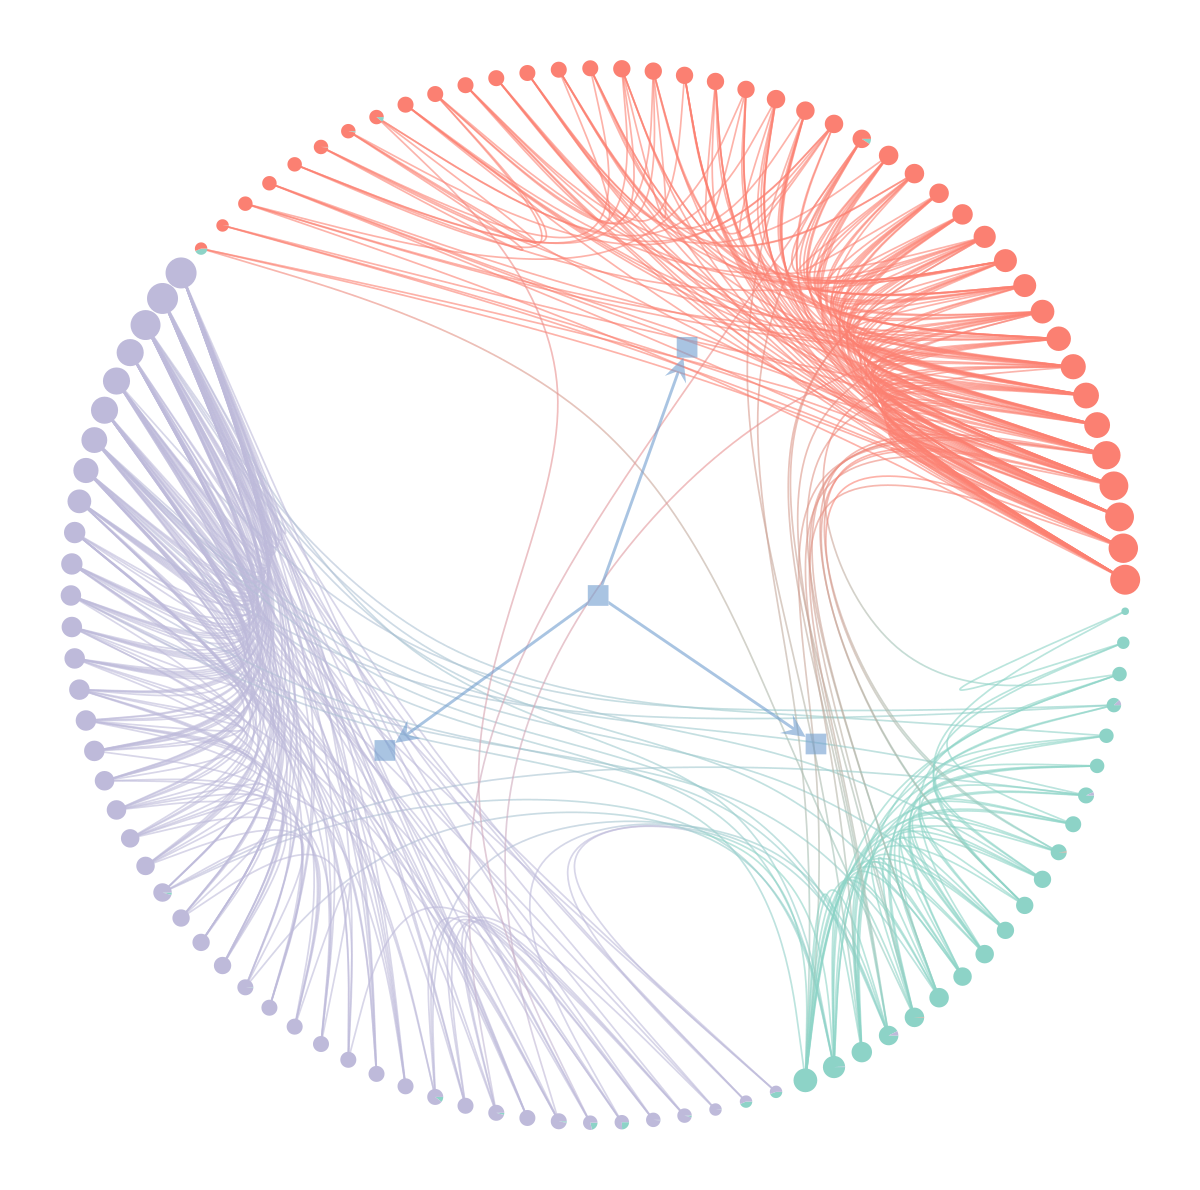
\includegraphics[width=\linewidth]{polbooks-graph.png}
				\caption{Polbooks $D=3$}
				\label{fig:polbooks-graph}
			\end{subfigure}
			\hfill
			\begin{subfigure}[t]{0.3\linewidth}
				\centering
				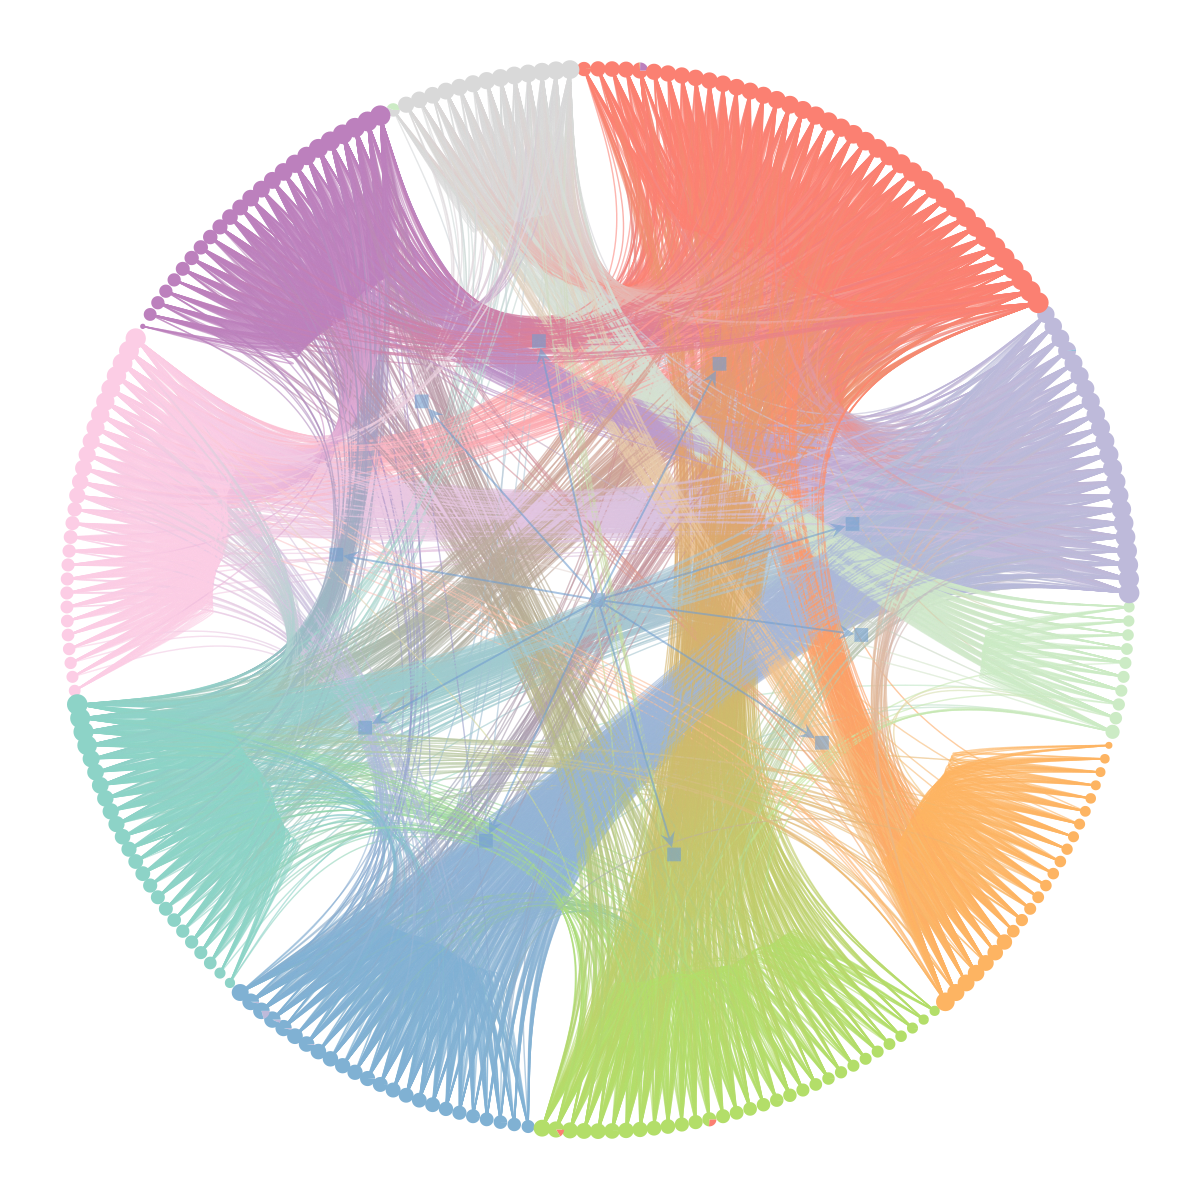
\includegraphics[width=\linewidth]{school-graph.png}
				\caption{school $D=13$}
				\label{fig:school-graph}
			\end{subfigure}
			\hfill
			\begin{subfigure}[t]{0.3\linewidth}
				\centering
				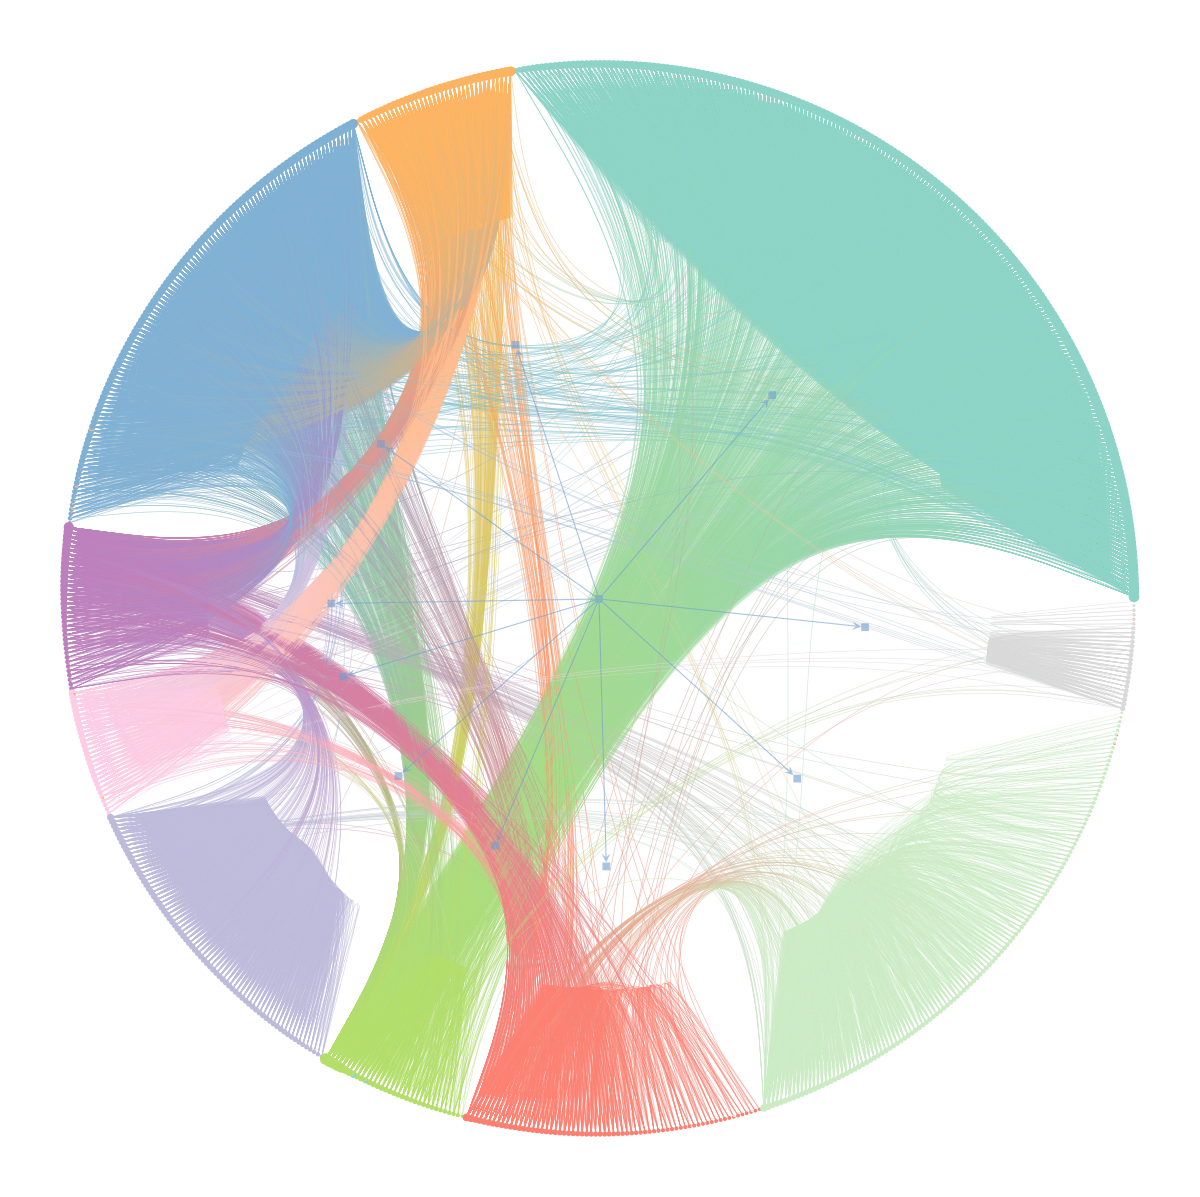
\includegraphics[width=\linewidth]{fb-graph.png}
				\caption{FB egonet $d=480$}
				\label{fig:fb-graph}
			\end{subfigure}
			\begin{subfigure}[t]{0.4\linewidth}
				\centering
				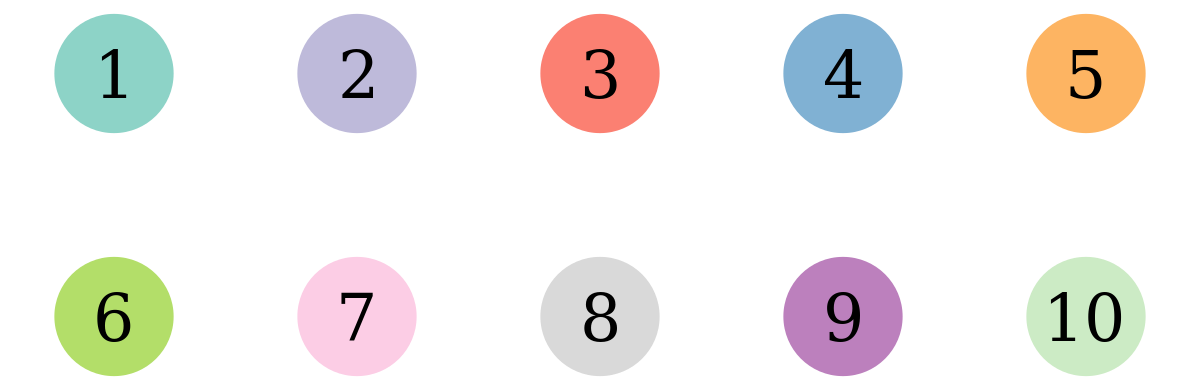
\includegraphics[width=0.8\linewidth]{10-horizontal-legend.png}
				\caption{Legend}
				\label{fig:10-legend}
			\end{subfigure}
			\caption{Networks laid out and coloured according to inferred block memberships $\hat{y}$ for a given experiment iteration. Visualisation performed using \textit{graph-tool} \cite{peixoto_graph-tool_2014}.}
			\label{fig:graphs-all}
		\end{figure}
	\end{frame}
	
	\begin{frame}{Political books \cite{polbooks}}
		\begin{figure}[!h]
			\centering
			\begin{subfigure}[t]{0.452\linewidth}
				\centering
				\vskip 0pt
				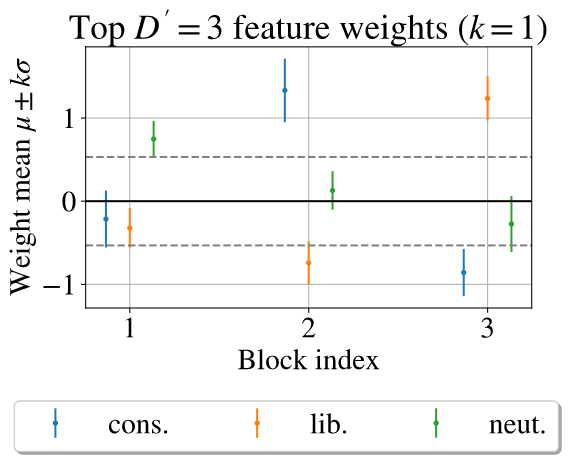
\includegraphics[width=\linewidth]{polbooks-null-1}
			\end{subfigure}
			\begin{subfigure}[t]{0.45\linewidth}
				\centering
				\vskip 0pt
				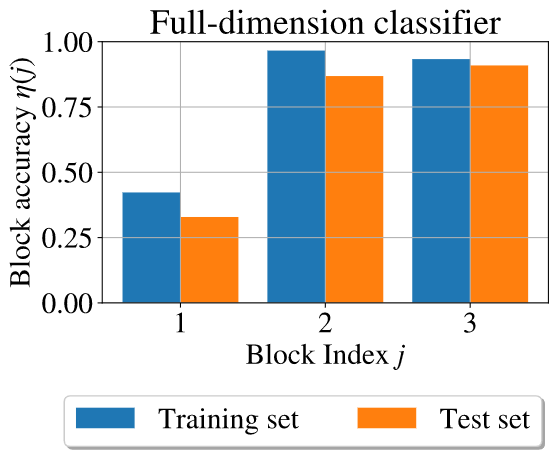
\includegraphics[width=\linewidth]{polbooks-accuracy-1}
			\end{subfigure}
		\end{figure}
		\begin{table}
			\centering
			\begin{tabular}{cc|cc}
				$B$ & $D$ & $\bar{\Lcal}_0$ & $\bar{\Lcal}_1$ \\ \hline
				3 & 3 & $0.563 \pm 0.042$ & $0.595 \pm 0.089$
			\end{tabular}
		\end{table}
	\end{frame}

\section{Conclusion}

	\begin{frame}{Conclusion}
		What have we achieved:
		\begin{itemize}
			\item Flip thinking of how we test for a feature's impact on graphical structure
			\item Developed efficient inference algorithm
		\end{itemize}
		What is yet to come:
		\begin{itemize}
			\item FFBM can only explain macro-structure $\Rightarrow$ extend to hierarchical structure
		\end{itemize}
		If I could start again
	\end{frame}

	
	\begin{frame}{Thanks for listening}
		\begin{figure}
			
\includegraphics[width=0.6\linewidth]{any-questions.jpg}
			\caption{Source, \citet{any-Qs}}
		\end{figure}

	\end{frame}

	\begin{frame}{References}
		\tiny
		\bibliography{presentation.bib}
	\end{frame}

\section*{Additional slides}

	\begin{frame}{Important property of the FFBM}
		\begin{theorem}
			Our prior choice for $p(\theta)$ gives us that,
			$$p(b|X) = B^{-N}.$$
		\end{theorem}
		
		Proof:
		\begin{align*}
			p(b | X) &= \int p(b | X, \theta) p(\theta) d\theta = \int \prod_{i \in [N] } \phi_{b_i}(x_i; \theta) p(\theta) d\theta \\
			&= \prod_{i \in [N]} \int \frac{\exp(w_{b_i}^T x_i) \prod_{j \in [B]} \Gaussian(w_j; 0, \sigma_\theta^2 I)}{\sum_{k \in [B]} \exp(w_{k}^T x_i)} dw_{1:B}.
		\end{align*}
		Which is a constant w.r.t. $b$.
	\end{frame}

	\begin{frame}{Metropolis-Hastings \cite{hastings-alg}}
		We want to draw samples $\left\{ z^{(t)} \right\}$ from some distribution,
		$$\pi^*(z) \propto \pi(z).$$
		Just need to be able to evaluate $\pi(z)$ point-wise and simulate from a proposal $q(z, z')$. If we accept each proposal with probability,
		$$\alpha(z, z') = \min \left( \frac{\pi(z') q(z', z)}{\pi(z) q(z, z')} , 1 \right),$$
		then the resulting Markov chain is in detailed balance with $\pi(z)$.
	\end{frame}
	
	\begin{frame}{$b$-step}
		Our target,
		$$p(b | A, X) \propto p(b | X) p(A | b) = \pi_b(b),$$
		can be evaluated as,
		\begin{align*}
			\pi_b(b) &= p(b|X) \sum_{\psi} p(A, \psi|b) \\
			&= p(b|X) p(A, \psi^* | b) \\
			&= p(A|\psi^*, b) p(\psi^*|b) p(b | X),
		\end{align*}
		where $\psi^*$ is the only value compatible with $(A,b)$. Big win for the microcanonical formulation.
		
		We borrow $q_b(b, b')$ from \citet{Peixoto-Bayesian-Microcanonical}.
	\end{frame}
	
	\begin{frame}{$\theta$-step}
		Our target can be written as:
		$$p(\theta | X, b) \propto
		{\color{blue} p(b |X, \theta)} 
		{\color{red}p(\theta)}
		= \pi_\theta(\theta) \propto \exp(-U(\theta)).$$
		$\therefore$ can write -ve log target as:
		$$U(\theta) 
		= {\color{blue} \sum_{i,j} y_{ij} \log \frac{1}{a_{ij}} } + 
		{\color{red} \frac{1}{2\sigma_\theta^2} || \theta ||^2} 
		= {\color{blue} N \Lcal(\theta)} 
		+ {\color{red} \frac{1}{2\sigma_\theta^2} ||\theta||^2 },$$
		
		where $y_{ij} \coloneqq \one \{b_i = j\}$ and $a_{ij} = \phi_{j}(x_i; \theta)$. This form looks very familiar? We can use $\nabla U$ to bias our proposal:
		$$\theta' = \theta^{(t)} - h_t \nabla U \left(\theta^{(t)} \right) + \sqrt{2h_t} \cdot \xi$$
		This is now called the Metropolis-adjusted Langevin algorithm (MALA).
	\end{frame}
	
	\begin{frame}{Serialise the chains}
		The $b^{(t)}$ does not use $\theta^{(t)}$.
		
		The $\theta^{(t)}$ update uses $b^{(t)}$ through $y^{(t)}_{ij} \coloneqq \one\{b^{(t)}_i = j\}$.
		
		Why not use empirical mean of this quantity:		
		$$\hat{y}_{ij} \coloneqq \frac{1}{|\Tcal_b|} \sum_{t \in \Tcal_b} y_{ij}^{(t)}.$$
		This is an unbiased estimate of $p(b_i=j|A,X)$.
		
		Using $\hat{y}$ instead of $y^{(t)}$ for the $\theta$-step:
		\begin{itemize}
			\item Reduced variance in evaluation of $U$ and $\nabla U$
			\item Can run $b$ and $\theta$-chains sequentially rather than in parallel $\Rightarrow$ different lengths.
		\end{itemize}
	\end{frame}

	\begin{frame}{Dimensionality Reduction}
		\begin{columns}
			\column{0.7\linewidth}
			Want to know which features we can discard:
			\begin{itemize}
				\item Write $\theta$ as matrix $W$, so that $W_{ij}$ is weight for block $i$ and feature $j$.
				\item Compute mean $\hat{\mu}_{ij}$ and std dev $\hat{\sigma}_{ij}$ of the $W_{ij}^{(t)}$-samples
			\end{itemize}
			Imagine a test on $W_{ij}$ such that:
			$$H_0: |W_{ij}| \leq c \qquad H_1: |W_{ij}| > c$$
			If we use Laplace approximation can come up with simple decision rule:
			$$h_{ij} = H_1 \iff \left(\hat{\mu}_{ij} - k \hat{\sigma}_{ij}, \hat{\mu}_{ij} + k \hat{\sigma}_{ij}\right)
			\cap (-c, +c) = \emptyset$$
			With $k>0$ controlling degree of significance of result
			\column{0.3\linewidth}
			\begin{figure}
				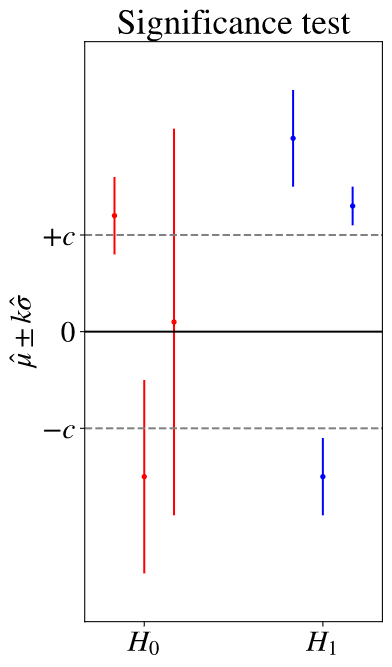
\includegraphics[width=\linewidth]{significance-test.png}
			\end{figure}
		\end{columns}		
	\end{frame}

	\begin{frame}{Dimensionality Reduction cont...}
		If we specify cut-off $c>0$ and multiplier $k>0$ can only retain features $d$ such that:
		$$\Dcal' \coloneqq \left\{ d \in [D] : \exists i \in [B] \textrm{ s.t. } h_{id} = H_1\right\}$$
		Instead it is often more practical to fix $|\Dcal'| = D'$ and $k=k_0$, then find the maximal cut-off:
		$$c^* = \argmax_{c>0}\{c: |\Dcal'|=D', k=k_0\}$$
	\end{frame}

	\begin{frame}{Primary school dynamic contacts \cite{schools}}
		\begin{figure}[!h]
			\centering
			\begin{subfigure}[t]{0.45\linewidth}
				\centering
				\imagebox{4.3cm}{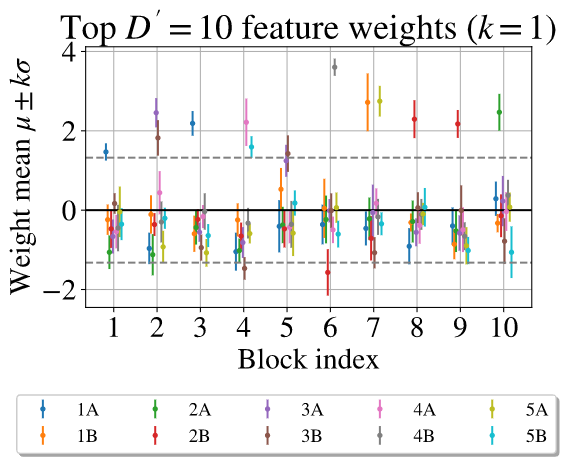
\includegraphics[width=\linewidth]{school-null-1}}
				\caption{$\theta$-samples. Dotted line is $\pm c^*$.}
			\end{subfigure}
			\begin{subfigure}[t]{0.45\linewidth}
				\centering
				\imagebox{4.3cm}{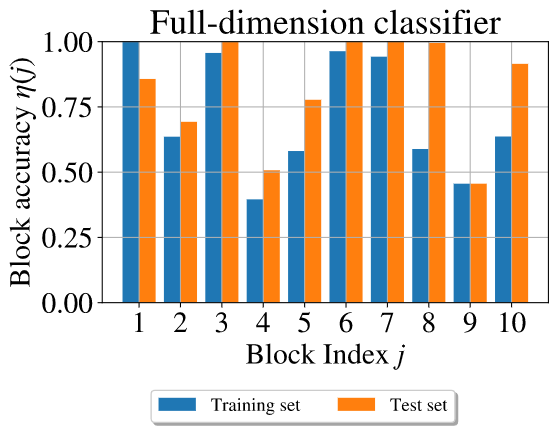
\includegraphics[width=\linewidth]{school-accuracy-1}}
			\end{subfigure}
		\end{figure}
		
		\begin{table}
			\centering
			\resizebox{\textwidth}{!}{%
				\begin{tabular}{ccc|cc|cc}
					$B$ & $D$ & $D'$ & $\bar{\Lcal}_0$ & $\bar{\Lcal}_1$ & $\bar{\Lcal}_0'$ & $\bar{\Lcal}_1'$ \\ \hline
					10 & 13 & 10 & $0.787 \pm 0.127$ & $0.885 \pm 0.129$ & $0.793 \pm 0.132$ & $0.853 \pm 0.132$
				\end{tabular}
			}
			\caption{Goodness of fit}
		\end{table}
	\end{frame}
	
	\begin{frame}{Facebook egonet \cite{fb-snap}}
		\begin{figure}[!h]
			\centering
			\begin{subfigure}[t]{0.45\linewidth}
				\centering
				\imagebox{4.9cm}{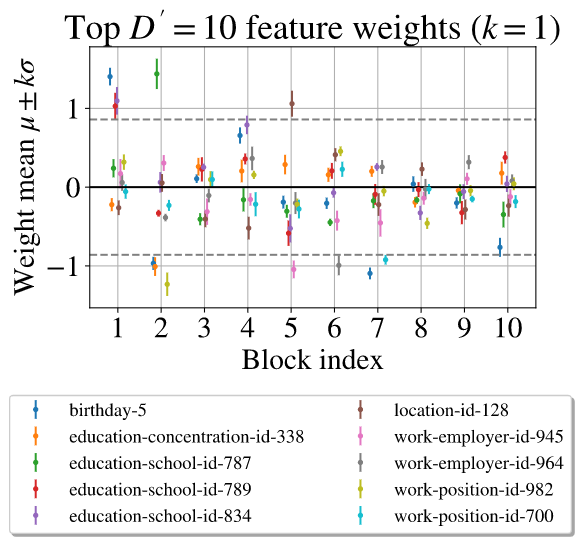
\includegraphics[width=\linewidth]{fb-null-1}}
			\end{subfigure}
			\begin{subfigure}[t]{0.45\linewidth}
				\centering
				\imagebox{4.9cm}{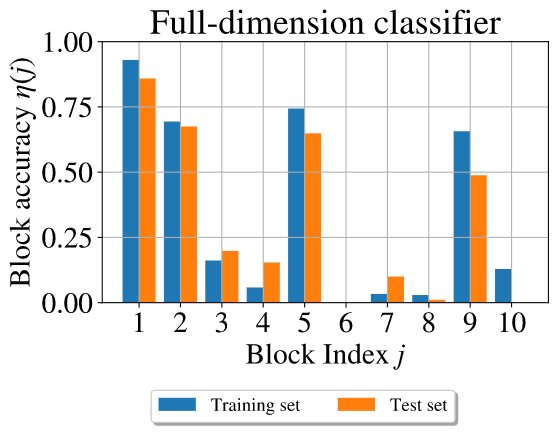
\includegraphics[width=\linewidth]{fb-accuracy-1}}
			\end{subfigure}
		\end{figure}
		
		\begin{table}
			\centering
			\resizebox{\textwidth}{!}{%
				\begin{tabular}{ccc|cc|cc}
					$B$ & $D$ & $D'$ & $\bar{\Lcal}_0$ & $\bar{\Lcal}_1$ & $\bar{\Lcal}_0'$ & $\bar{\Lcal}_1'$ \\ \hline
					10  & 480 & 10 & $1.326 \pm 0.043$ & $1.538 \pm 0.069$ & $1.580 \pm 0.150$ & $1.605 \pm 0.106$
				\end{tabular}
			}
			\caption{Goodness of fit}
		\end{table}
	\end{frame}

\end{document}
